\subsection{Memory Resistor}
\label{sec:current_capabilities_memory_resistor}

Several independent research groups have been exploring how to make use of memristors to build artificial synapses \cite{ahah,memristor_conditioning}. The efficiency of a synapse may essentially be encoded as the resistance of a memristor, and synaptic networks may thus be built using several memristors, where neural activity will strive for the path of least resistance.

%Robin.

An experiment was conducted in 2010, which used memristors as artificial synapses to empirically validate the formation of associative memories between three neurons and two synapses (see figure \ref{fig:conditioning_with_artificial_synapses}). In the experiment, two input neurons and one output neuron was used. The input neurons were connected to the output neuron, using one artificial synapse each. When the input neurons were triggered at the same time, their activity became associated to each other, as the resistance of their memristors decreased. This made it possible to activate one neuron, simply by activating the other, which may be compared to the classical experiment by Pavlov where dogs were conditioned to salivate when presented with triggering stimuli, e.g. the sound of a bell.

\begin{figure}[htbp]
	\begin{center}
		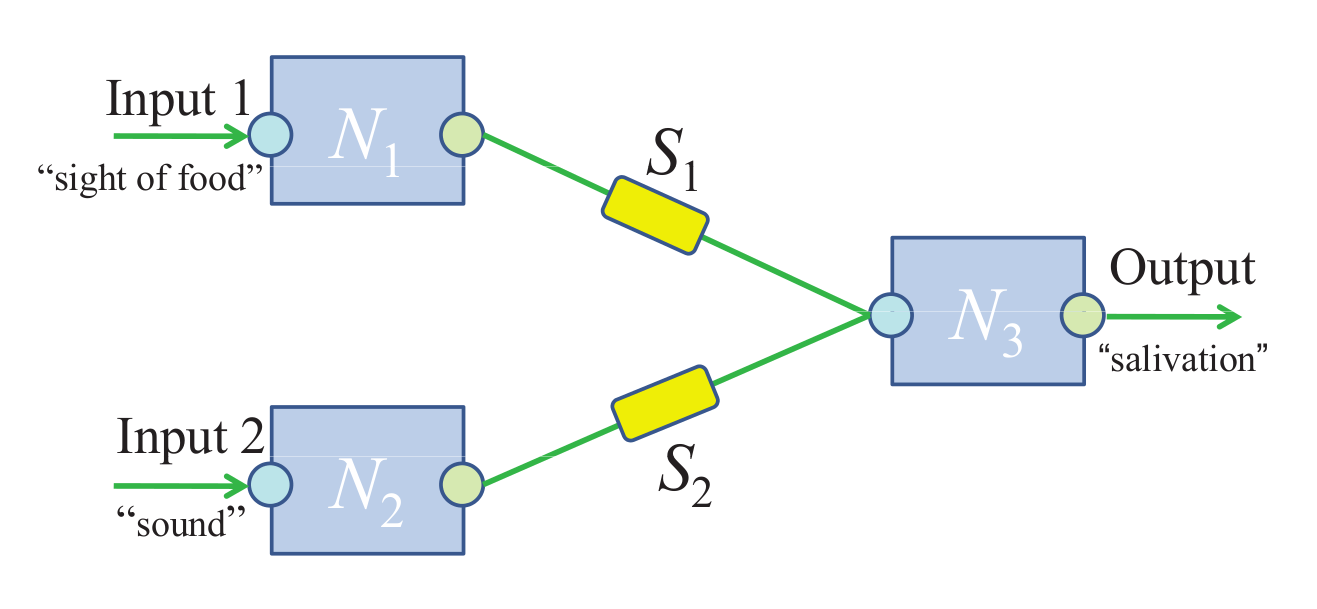
\includegraphics[width=0.5\textwidth]{inc/conditioning_with_artificial_synapses.png}
		\caption{Associative memory formation (in the form of traditional conditioning) achieved using artificial synapses.\protect\footnotemark}
		\label{fig:conditioning_with_artificial_synapses}
	\end{center}
\end{figure}
\footnotetext{Original image (© Yuriy V. Pershin and Massimiliano Di Ventra): \url{https://arxiv.org/pdf/0905.2935.pdf}}


%The experiment was based on Hebb's rule, and , that \textit{``cells which fire together, wire together''}  \cite{memristor_conditioning}.

%ref: http://www.hpl.hp.com/news/2008/apr-jun/memristor.html
%
% > "The memristor could lead to far more energy-efficient computers with some of the pattern-matching abilities of the human brain.
% > - Jamie Beckett, April 2008
